\documentclass[]{article}
\usepackage{graphicx}
\graphicspath{ {media/} }

% Title Page
\title{Lane Line Finding Project Writeup}

\begin{document}
\maketitle

\section{Project Goal}
The goal of this project is to build a basic computer vision pipeline to identify and mark lane lines on static images and video streams taken from a car-mounted camera. The pipeline should be able to locate the lines of the left and right lane, extrapolate them to a full straight line and then mark them as an overlay on the original image or video.


\section{Processing Pipeline}
The processing pipeline is divided into four steps: image preprocessing, segment identification, line extrapolation and overlay drawing. Most of the pipeline is contained in the \textit{draw\_lane\_lines()} function, although some later improvements are implemented outside of it.


\paragraph{Image Preprocessing}
In this step, the original image is first resized to a standard size, then converted to grayscale, and finally blurred with some Guassian noise. Ideally, the pipeline should be able to work with arbitrary-sized input images. However, we chose to convert the image to a standard size for two reasons:
\begin{enumerate}
	\item The parameters of segment identification step depend on the pixel density of the input image, therefore fixing the input image size ensures that the algorithm performs as expected regardless of input resolution.
	\item The bounding box also depends on the resolution of input images. We could use relative coordinates (e.g. 0.3 * image width) for the bounding boxes, but a fixed-sized input is more convenient.
\end{enumerate}
Grayscale is applied because the processings in the next step do not utilise colour channel information.
Finally, Gaussian noise helps smooth out the results of Canny edge detection in the next step.

\paragraph{Segment Identification}
In this step, we apply two OpenCV functions consecutively to extract the line segments of the lane lines from the images. We first use the \textit{canny()} helper function to apply Canny edge detection, then select the interested region with the \textit{region\_of\_interest()} helper function, and finally apply the \textit{cv2.HoughLinesP()} function to extract line segments from the detected edges using Hough transform. The \textit{hough\_lines()} helper function is not used because we would like to extrapolate a line from the segments, rather than directly overlaying the segments on the input images.

\begin{figure}[h]
	\centering
	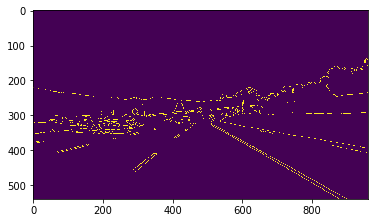
\includegraphics[width=0.5\textwidth]{canny}
	\caption{Canny Edge Detection}
\end{figure}

\begin{figure}[h]
	\centering
	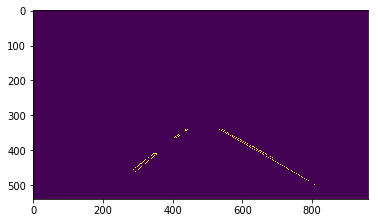
\includegraphics[width=0.5\textwidth]{canny_bound}
	\caption{Bounded Edge Detection}
\end{figure}

\begin{figure}[h]
	\centering
	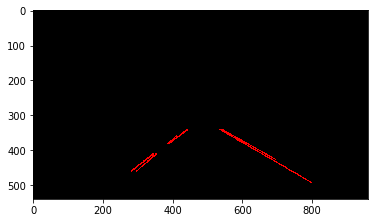
\includegraphics[width=0.5\textwidth]{hough}
	\caption{Segment Detection with Hough Transform}
\end{figure}

\paragraph{Line Extrapolation}
In this step, we follow the substeps below to obtain the lines of the left and right lane:
\begin{enumerate}
	\item Calculate the inclination angles (using arctan) of each line segment returned by the Hough transform algorithm;
	\item Filter the segments to remove apparently horizontal segments (which are unlikely to be lane lines);
	\item Separate the segments of left and right lanes by their inclination angles (they should be of different signs);
	\item Calculate the weighted average of the inclination angle and segment starting position for left and right lane respectively, weighted by the segment lengths;
	\item Use trigonometry to calculate the start and end points of the left and right lane lines.
\end{enumerate}
The reason we need to calculate the inclination angle in substep 1 despite only using tangents in substep 5 is that tangents (or slopes) cannot be simply averaged. The weighted average step puts more confidence in longer segments in combat possible detection artefacts.

\paragraph{Overlay Drawing}
In this step, we simply draw the lines from the last step and overlay them on top of the input image with the helper function \textit{weighted\_img()}. The scaling from step 1 is also taken into account.

\section{Potential Shortcomings}

One immediate observation from the outputs is that the detected lane lines are very jittery and unstable in video outputs. Lowering the sensitivity of Canny and Hough transform algorithms helps, but it also causes the detection of the dashed lane lines to be lost in some frames. Here, we apply exponetial smoothing to try and combat this. Instead of applying a stateless \textit{process\_image()} function to each video frames, we create a Python class with a \textit{process\_image()} method. This class remembers the (smoothed) inclination angles and x-intercepts from the last frame and applies exponential smoothing to newly calculated line positions. When the detection is lost at one frame, the last known location of the lane line is used in the output. This greatly improves the stability of lane detection and adds some robustness against small interferences in the input. However, too much smoothing causes detection of real changes to lag behind, and therefore it should be applied with care.

The current pipeline is very weak and unreliable when dealing with turns and especially curved lanes. The lane separation is done with inclination angles, however when turning a vehicle, the lanes may appear to have the same direction of inclination, or even parallel, therefore breaking the current lane separation algorithm. Also, the line detection algorithm is not able to deal with lanes with large curvatures, and line extrapolation will not make sense in that scenario.

Another issue is that sometimes non-lane lines can be detected in the original image, such as horizontal seams between concrete blocks in the "challenge" video. Angle filtering helps with removing horizontal lines with small angles, but it does not work every time. As we see in figure \ref{fig:intrf}, even with smoothing, the interference is still significant.

\begin{figure}[h]
	\centering
	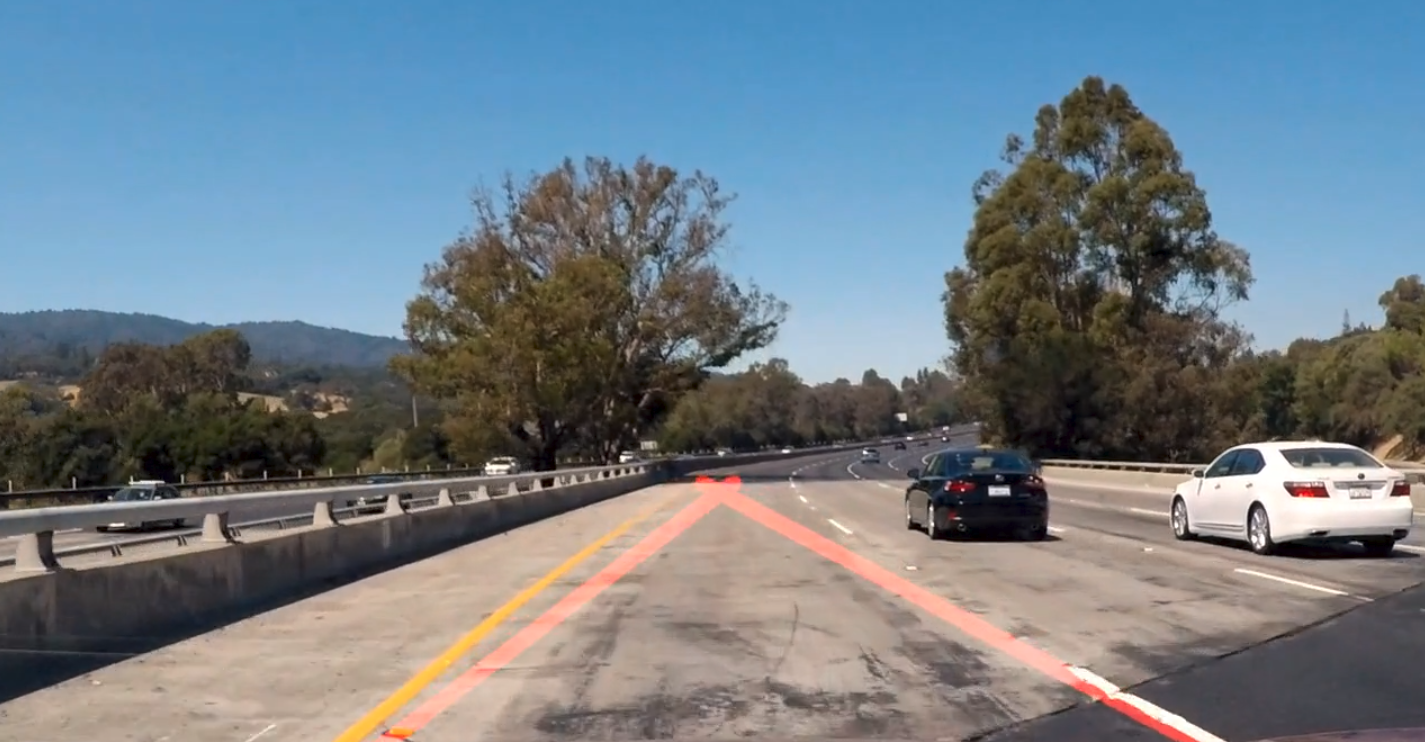
\includegraphics[width=0.7\textwidth]{issue}
	\caption{Beginning of Concrete Bridge Interferring with Lane Finding}
	\label{fig:intrf}
\end{figure}

\section{Suggested Improvements}

To obtain more stable outputs, we may augment exponential smoothing with a probabilistic model which calculates how likely the current frame output is valid given the last frame, and rejects outputs that are very unlikely / almost certainly artefacts.

The separation of lanes with inclination angles only works when the camera position is sufficiently low and the turning angle of the vehicle is sufficiently small. This is not robust in real driving situations. We could apply perspective transforms to remove the effect of relative postions between camera, car and the lanes on lane detection and separation.

We will need more than line segment detection to deal with curved lanes. Some form of curve detection is necessary.

We also have not taken into account the colour channels in the edge / segment detection step. In reality, colour is useful for distinguishing real lane lines from other lines on the road, as well as defending against interferences such as shadows. More advanced algorithms should fully utilise the colour information.

\end{document}          
